\section{液体对压强的传递}\label{sec:5-3}


液体能够流动。由于液体具有流动性,所以在受到压力的时候,就出现跟固体不同的现象。下面我们就来研究这个问题。

取一个壁上有几个小孔的空心球,球上连接一个圆筒,每一个小孔上都扎有橡皮膜。把水倒进球和筒里,用活塞压筒里的水,
可以看到,扎在各个小孔上的橡皮膜都向外凸出(图 \ref{fig:5-8})。这表明活塞加在水上的压强,被水传递到了各个小孔的橡皮膜上。
球上的小孔是朝着不同方向的,可见,\CJKunderwave{液体能够把它受到的压强向各个方向传递}。

\begin{figure}[htbp]
    \centering
    \begin{minipage}{6cm}
    \centering
    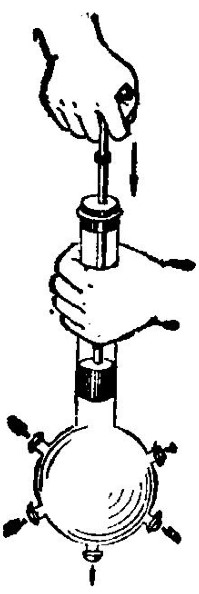
\includegraphics[width=2cm]{../pic/czwl1-ch5-8}
    \caption{}\label{fig:5-8}
    \end{minipage}
    \qquad
    \begin{minipage}{8cm}
    \centering
    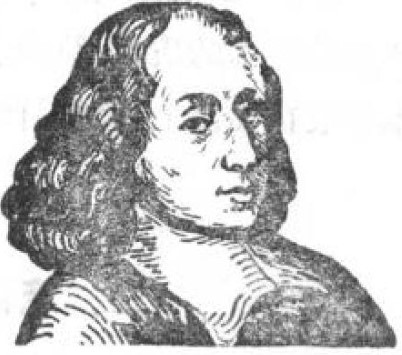
\includegraphics[width=4cm]{../pic/czwl1-ch5-9}
    \caption*{帕斯卡(1623 ~ 1662)}\label{fig:5-pascal}
    \end{minipage}
\end{figure}

水龙带没有灌水时是扁的,接到水龙头上灌满水后成圆柱形,就是因为水龙头里出来的水用很大的压强压带里的水,
这个压强被水传递到水龙带壁的各个部分的缘故。

十七世纪,法国科学家帕斯卡用实验的方法,仔细研究了液体传递压强的问题。
他发现密闭液体向各个方向传递的压强,等于外力加在液体上的压强。
从而得出了液体传递压强的规律:
\textbf{加在密闭液体上的压强,能够大小不变地被液体向各个方向传递}。
这个规律叫做\textbf{帕斯卡定律}。


